% Options for packages loaded elsewhere
\PassOptionsToPackage{unicode}{hyperref}
\PassOptionsToPackage{hyphens}{url}
\PassOptionsToPackage{dvipsnames,svgnames,x11names}{xcolor}
%
\documentclass[
]{article}

\usepackage{amsmath,amssymb}
\usepackage{iftex}
\ifPDFTeX
  \usepackage[T1]{fontenc}
  \usepackage[utf8]{inputenc}
  \usepackage{textcomp} % provide euro and other symbols
\else % if luatex or xetex
  \usepackage{unicode-math}
  \defaultfontfeatures{Scale=MatchLowercase}
  \defaultfontfeatures[\rmfamily]{Ligatures=TeX,Scale=1}
\fi
\usepackage{lmodern}
\ifPDFTeX\else  
    % xetex/luatex font selection
  \setmainfont[]{Latin Modern Roman}
\fi
% Use upquote if available, for straight quotes in verbatim environments
\IfFileExists{upquote.sty}{\usepackage{upquote}}{}
\IfFileExists{microtype.sty}{% use microtype if available
  \usepackage[]{microtype}
  \UseMicrotypeSet[protrusion]{basicmath} % disable protrusion for tt fonts
}{}
\makeatletter
\@ifundefined{KOMAClassName}{% if non-KOMA class
  \IfFileExists{parskip.sty}{%
    \usepackage{parskip}
  }{% else
    \setlength{\parindent}{0pt}
    \setlength{\parskip}{6pt plus 2pt minus 1pt}}
}{% if KOMA class
  \KOMAoptions{parskip=half}}
\makeatother
\usepackage{xcolor}
\setlength{\emergencystretch}{3em} % prevent overfull lines
\setcounter{secnumdepth}{5}
% Make \paragraph and \subparagraph free-standing
\ifx\paragraph\undefined\else
  \let\oldparagraph\paragraph
  \renewcommand{\paragraph}[1]{\oldparagraph{#1}\mbox{}}
\fi
\ifx\subparagraph\undefined\else
  \let\oldsubparagraph\subparagraph
  \renewcommand{\subparagraph}[1]{\oldsubparagraph{#1}\mbox{}}
\fi


\providecommand{\tightlist}{%
  \setlength{\itemsep}{0pt}\setlength{\parskip}{0pt}}\usepackage{longtable,booktabs,array}
\usepackage{calc} % for calculating minipage widths
% Correct order of tables after \paragraph or \subparagraph
\usepackage{etoolbox}
\makeatletter
\patchcmd\longtable{\par}{\if@noskipsec\mbox{}\fi\par}{}{}
\makeatother
% Allow footnotes in longtable head/foot
\IfFileExists{footnotehyper.sty}{\usepackage{footnotehyper}}{\usepackage{footnote}}
\makesavenoteenv{longtable}
\usepackage{graphicx}
\makeatletter
\def\maxwidth{\ifdim\Gin@nat@width>\linewidth\linewidth\else\Gin@nat@width\fi}
\def\maxheight{\ifdim\Gin@nat@height>\textheight\textheight\else\Gin@nat@height\fi}
\makeatother
% Scale images if necessary, so that they will not overflow the page
% margins by default, and it is still possible to overwrite the defaults
% using explicit options in \includegraphics[width, height, ...]{}
\setkeys{Gin}{width=\maxwidth,height=\maxheight,keepaspectratio}
% Set default figure placement to htbp
\makeatletter
\def\fps@figure{htbp}
\makeatother
\newlength{\cslhangindent}
\setlength{\cslhangindent}{1.5em}
\newlength{\csllabelwidth}
\setlength{\csllabelwidth}{3em}
\newlength{\cslentryspacingunit} % times entry-spacing
\setlength{\cslentryspacingunit}{\parskip}
\newenvironment{CSLReferences}[2] % #1 hanging-ident, #2 entry spacing
 {% don't indent paragraphs
  \setlength{\parindent}{0pt}
  % turn on hanging indent if param 1 is 1
  \ifodd #1
  \let\oldpar\par
  \def\par{\hangindent=\cslhangindent\oldpar}
  \fi
  % set entry spacing
  \setlength{\parskip}{#2\cslentryspacingunit}
 }%
 {}
\usepackage{calc}
\newcommand{\CSLBlock}[1]{#1\hfill\break}
\newcommand{\CSLLeftMargin}[1]{\parbox[t]{\csllabelwidth}{#1}}
\newcommand{\CSLRightInline}[1]{\parbox[t]{\linewidth - \csllabelwidth}{#1}\break}
\newcommand{\CSLIndent}[1]{\hspace{\cslhangindent}#1}

\usepackage{hyphenat}
\makeatletter
\makeatother
\makeatletter
\makeatother
\makeatletter
\@ifpackageloaded{caption}{}{\usepackage{caption}}
\AtBeginDocument{%
\ifdefined\contentsname
  \renewcommand*\contentsname{Table of contents}
\else
  \newcommand\contentsname{Table of contents}
\fi
\ifdefined\listfigurename
  \renewcommand*\listfigurename{List of Figures}
\else
  \newcommand\listfigurename{List of Figures}
\fi
\ifdefined\listtablename
  \renewcommand*\listtablename{List of Tables}
\else
  \newcommand\listtablename{List of Tables}
\fi
\ifdefined\figurename
  \renewcommand*\figurename{Figure}
\else
  \newcommand\figurename{Figure}
\fi
\ifdefined\tablename
  \renewcommand*\tablename{Table}
\else
  \newcommand\tablename{Table}
\fi
}
\@ifpackageloaded{float}{}{\usepackage{float}}
\floatstyle{ruled}
\@ifundefined{c@chapter}{\newfloat{codelisting}{h}{lop}}{\newfloat{codelisting}{h}{lop}[chapter]}
\floatname{codelisting}{Listing}
\newcommand*\listoflistings{\listof{codelisting}{List of Listings}}
\makeatother
\makeatletter
\@ifpackageloaded{caption}{}{\usepackage{caption}}
\@ifpackageloaded{subcaption}{}{\usepackage{subcaption}}
\makeatother
\makeatletter
\makeatother
\ifLuaTeX
  \usepackage{selnolig}  % disable illegal ligatures
\fi
\IfFileExists{bookmark.sty}{\usepackage{bookmark}}{\usepackage{hyperref}}
\IfFileExists{xurl.sty}{\usepackage{xurl}}{} % add URL line breaks if available
\urlstyle{same} % disable monospaced font for URLs
\hypersetup{
  pdftitle={Network modularity is widely misused in ecological analyses},
  colorlinks=true,
  linkcolor={blue},
  filecolor={Maroon},
  citecolor={Blue},
  urlcolor={Blue},
  pdfcreator={LaTeX via pandoc}}





\title{ { Network modularity is widely misused in ecological analyses}}
\author{
{Michael D. Catchen}\textsuperscript{%
1,2,%
3%
}%
}




\date{}

\usepackage{setspace}
\usepackage[left,pagewise]{lineno}
\usepackage[letterpaper]{geometry}

\singlespacing
\geometry{lmargin=3cm}
\geometry{rmargin=4.5cm}

\begin{document}

%\setsansfont{Roboto}
%\setmathfont{TeX Gyre Termes Math}[version=termes]
\setstretch{1.15}



\parbox{14cm}{\setstretch{0.9}\raggedright\bfseries\huge\nohyphens{Network
modularity is widely misused in ecological analyses}}

\vskip 1em
\normalsize 
{Michael D. Catchen}\textsuperscript{%
1,2,%
3%
}%


\vskip 2em
{\normalsize\centering
\textbf{Abstract} Stop using modularity maximization.
\vskip 1em
}
\vskip 4em
%\flushleft
\raggedright
\hypertarget{introduction}{%
\section{Introduction}\label{introduction}}

Ecosystems are composed of interactions between species and their
environment. These interactions form networks that enable the
persistence of species, ecosystems, and the services ecosystems provide
people. In the last few decades, \emph{network science} has developed to
understand networks across a variety of domains. This field has
developed numerous quantitative tools for describing network structure,
which have seen increasing adoption in ecosystem science in the
burgeoning subfield of network ecology (Delmas \emph{et al.} 2019). One
such property is \emph{modularity} (denoted \(Q\)), which is a metric
that describes ``how well'' nodes of a network can be grouped into
\emph{modules}, first introduced in Newman \& Girvan (2004). Modularity
has been widely adopted as a metric of interest in ecological networks,
and in principle the grouping of species into modules could contain
biologically meaningful information.

Unfortunately, the most popular method identifying modules in ecological
networks is Modularity Maximization (MM), which has many well documented
flaws for robustly identifying modules in networks (Fortunato \&
Barthélemy 2007; Good \emph{et al.} 2010; Lancichinetti \& Fortunato
2011; Peixoto 2021). Still, MM is widely used in network ecology. In a
brief literature survey, we found MM methods overwhelmingly prevelent in
the analysis of ecological networks. Here we cover what modularity
maximization is, and why it doesn't work for identifying modules/groups
in networks. We suggest methods for community detection based on
Stochastic Block Models (Karrer \& Newman 2011; Peixoto 2014; Yen \&
Larremore 2020) for identifying modules in ecological networks.

\hypertarget{what-is-modularity}{%
\section{What is modularity?}\label{what-is-modularity}}

Consider an undirected network defined by an adjacency matrix
\(\mathbf{A}\), where \(A_{ij} = 1\) if nodes \(i\) and \(j\) share an
edge, and \(0\) otherwise. Let \(m = \sum_{i,j} A_{ij}\) denote the
total number of edges in the network, and \(k_i\) be the degree (the
number of edges) associated with node \(i\). Let \(b_i\) denote the
\emph{group} (or module) that node \(i\) belongs to. Modularity (\(Q\))
is then defined as

\[Q = \frac{1}{2m} \sum_{i,j} \bigg( A_{ij} - \frac{k_i k_j}{2m}\bigg)
\delta(b_i, b_j)\]

where \(\delta\) is a function that equals \(1\) if \(b_i = b_j\), and
equals \(0\) otherwise. It is essential to emphasize that
\textbf{modularity is not a property of a network \emph{alone}}. It is
only defined for a network \emph{and a set of group assignments for each
node}, \(\vec{b}\).

This value can be interpreted intuitively as how many more edges exist
between members of the same group than would be expected if edges were
distributed ``at random''. As pointed out by Peixoto (2021), there is an
implicit null model in what ``at random'' means in this definition,
namely the Chung-Lu configuration model (Chung \& Lu 2002), where the
probability of an edge existing between nodes \(i\) and \(j\) is
\(\mathbb{E}[A_{ij}] = \frac{k_i k_j}{2m}\).

\hypertarget{what-is-modularity-maximization}{%
\section{What is modularity
maximization?}\label{what-is-modularity-maximization}}

Modularity maximization (MM) is one of many potential methods for the
problem of taking an observed network \(\mathbf{A}\) and infering which
group \(b_i\) each node \(i\) belongs to (in network science literature,
this problem is called \emph{community detection}). MM originated during
the mid-2000s (Newman \& Girvan 2004) and was popularized through the
efficeincy of the Clauset-Newman-Moore (CNM) algorithm (Clauset \emph{et
al.} 2004) and the Louvain algorithm (Blondel \emph{et al.} 2008), both
of which made implementation of MM feasible for very large networks (at
the time, hundreds or thousands of nodes). Six years later after its
proposal, Good \emph{et al.} (2010) (with Clauset, architect of CNM, as
senior author) showed that in practice communities identified via
modularity maximization are fataly flawed for all but idealized
networks, and advocated against its use in ``in all but the most
straightforward cases''. More recently, Peixoto (2021) more thoroughly
explores this issue, showing how MM can massively overfit and find
highly modular partitions (\(Q \approx 0.5\)) in networks with no
modular structure.

\hypertarget{why-doesnt-modularity-maximization-work}{%
\section{Why doesn't modularity maximization
work?}\label{why-doesnt-modularity-maximization-work}}

As pointed out by Peixoto (2021), modularity maximization fails on two
fronts: it simultaneously \emph{overfits} (by finding clusters that have
high modularity \(Q\) but are entirely sporatic and unrelated to the
mechanisms by which the network was generated) and \emph{underfits} (by
having a limit on the size of what communities are recoverable relative
to the size of the whole network, called the \emph{resolution limit}
(Fortunato \& Barthélemy 2007)).

\hypertarget{overfitting-via-a-poor-choice-of-objective-function}{%
\subsection{Overfitting via a poor choice of objective
function}\label{overfitting-via-a-poor-choice-of-objective-function}}

Degeneracy of the modularity function, lots of very similar local optima
across widely different group partitions.

``The magnitude of the degeneracy problem, and the dependence of
\(Q_{max}\) on the size and number of modules in the network, suggests
that modules identified through modularity maximization should be
treated with caution in all but the most straightforward cases.'' Good
\emph{et al.} (2010).

\begin{figure}

{\centering 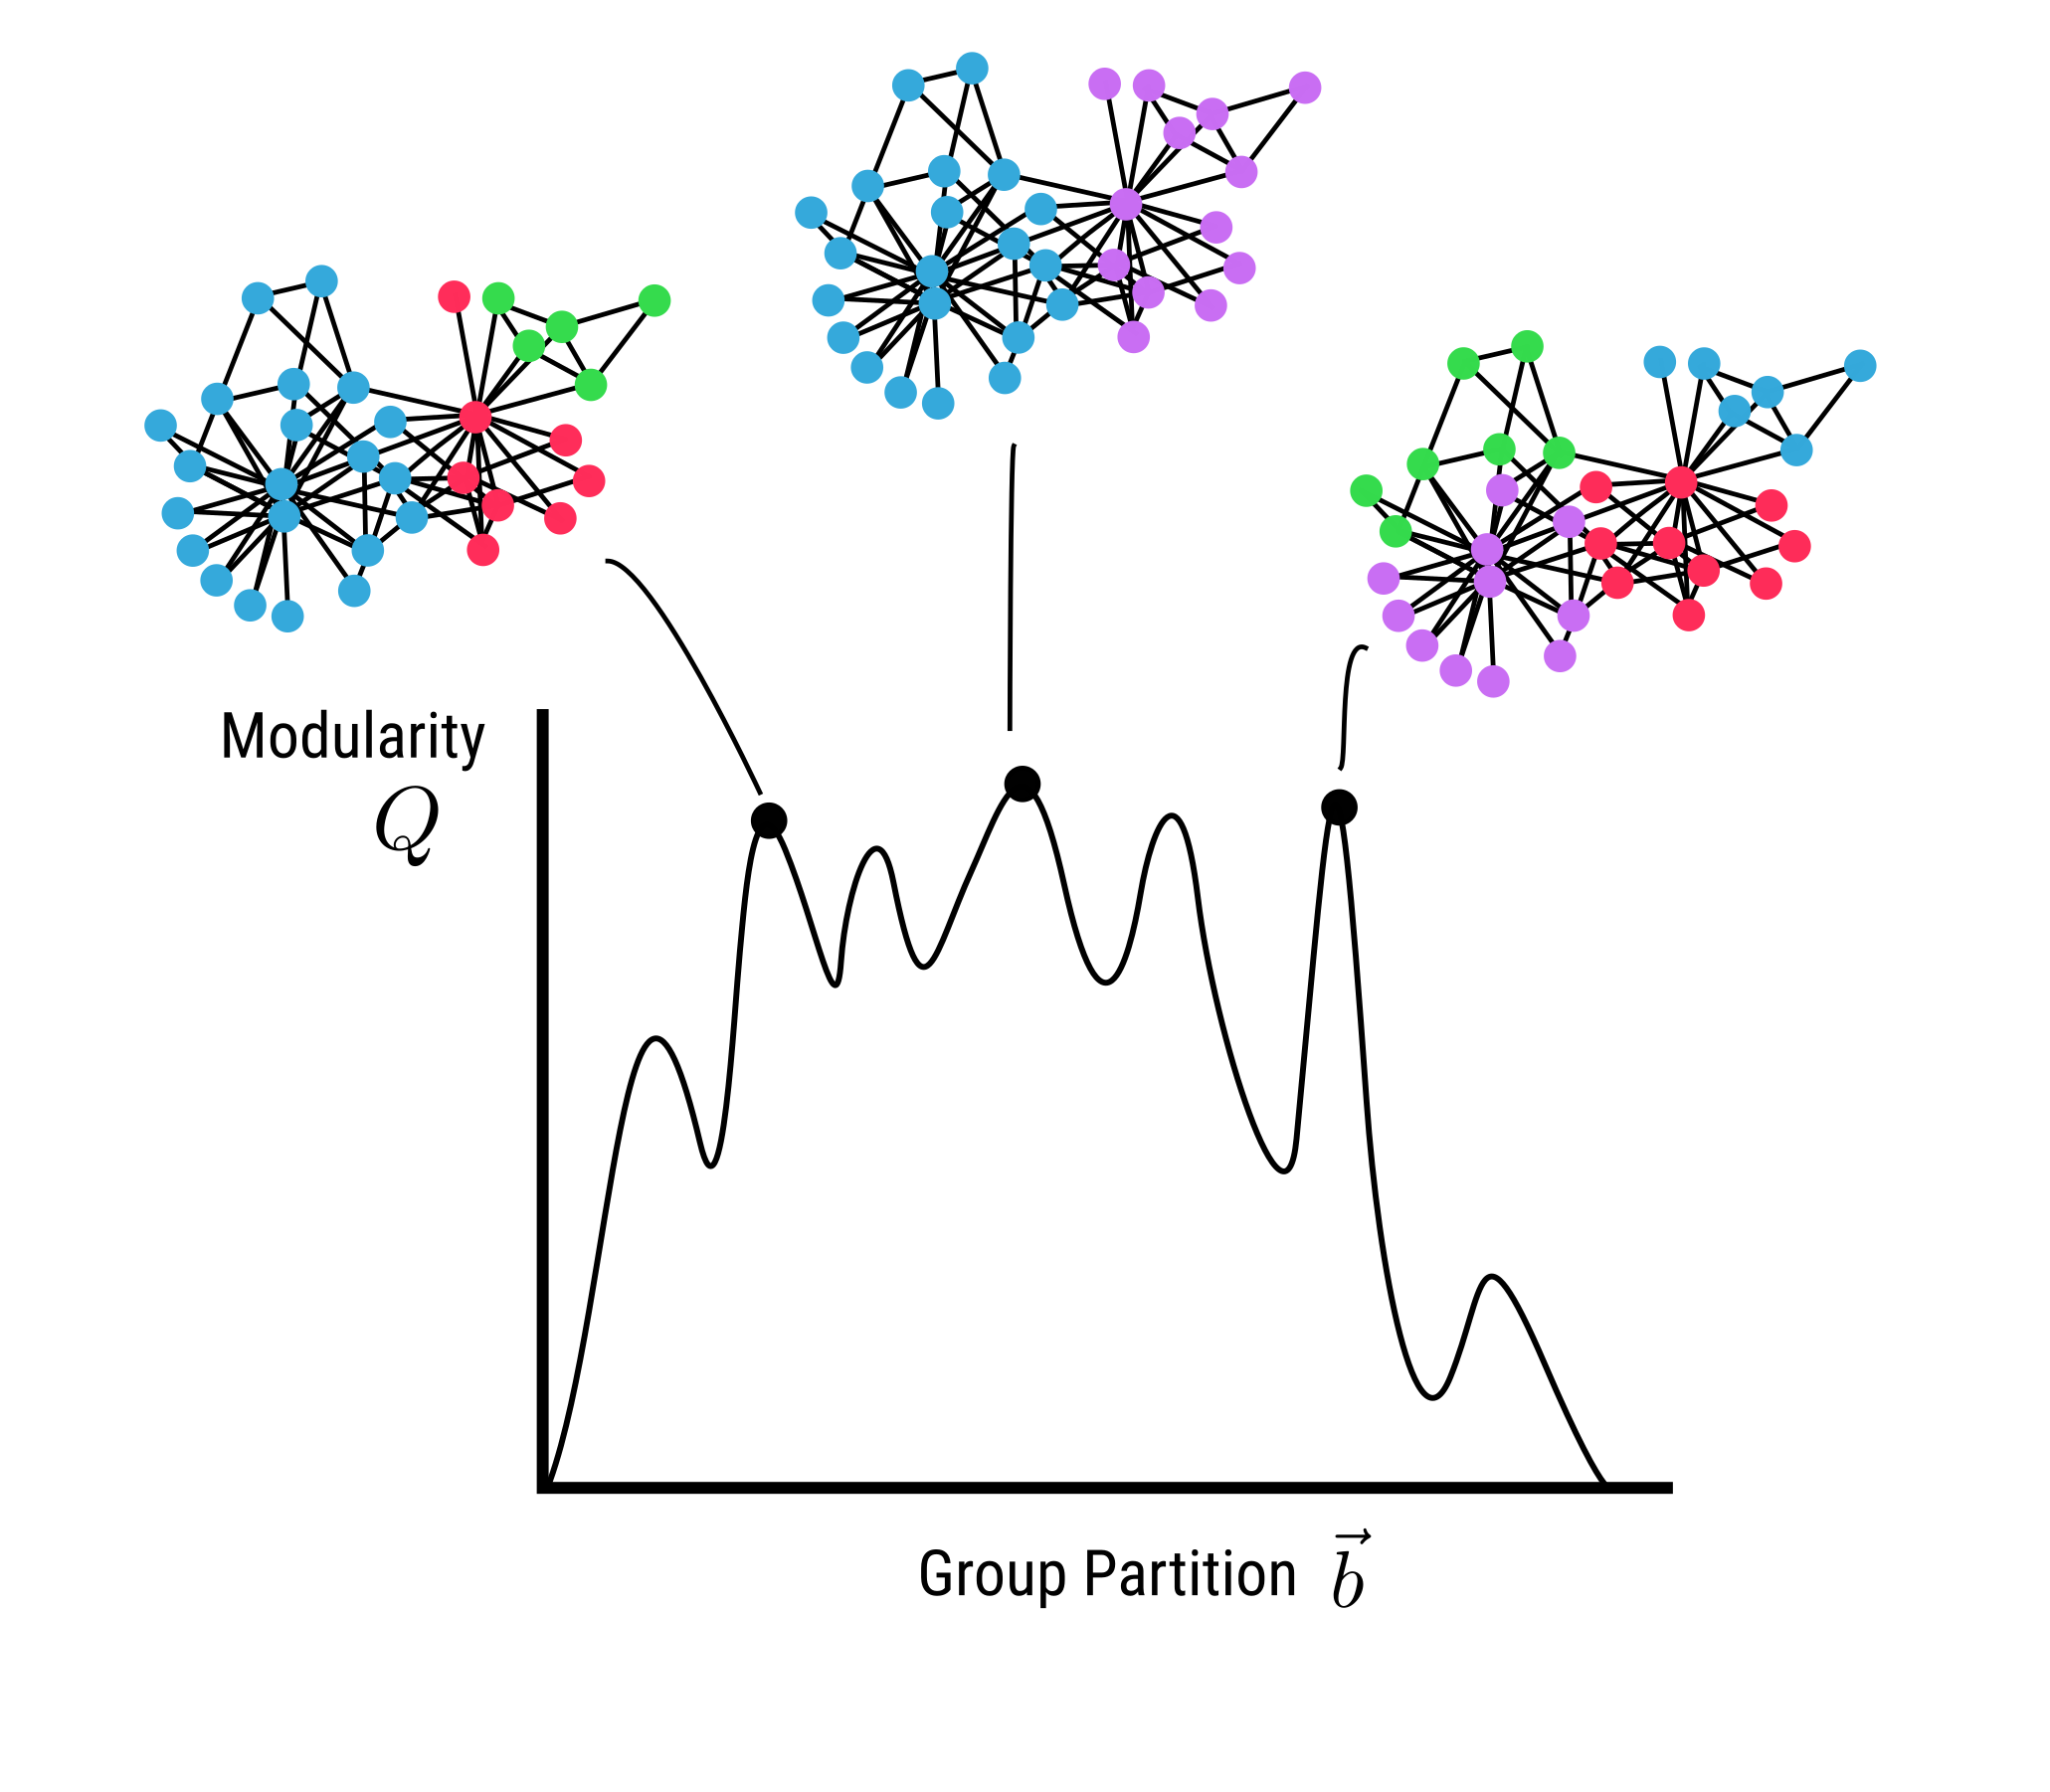
\includegraphics{figures/bumpy.png}

}

\caption{\label{fig-embedding}The issue with modularity maxmimization:
there are many local optima with similar \(Q\) values that correspond to
qualitatively very different group partitions.}

\end{figure}

\hypertarget{underfitting-via-the-resolution-limit}{%
\subsection{Underfitting via the resolution
limit}\label{underfitting-via-the-resolution-limit}}

The second issue with modularity maximization is that is cannot identify
communities that at smaller than a certain size. The threshold for
smallest community identifiable via MM is a function of the total size
over the network, and called the ``resolution limit'' in the network
science literature (Fortunato \& Barthélemy 2007; Lancichinetti \&
Fortunato 2011).

\hypertarget{modularity-maximization-is-rampant-in-ecological-network-studies}{%
\section{Modularity maximization is rampant in ecological network
studies}\label{modularity-maximization-is-rampant-in-ecological-network-studies}}

We found in a survey of 50+ papers on ecological networks, modularity
maximization is extremely common as the method for finding communities.
The goal of this paper is not to shame or call-out specific papers, but
to highlight that a widely adopted practice has fundemental flaws, and
to advocate a principle alternative for community detection.

We suspect MM is so prolific because it is widely available in many
packages for network analysis, including \texttt{bipartite}, which uses
a method for modularity maximization for bipartite networks proposed by
Dormann \& Strauss (2014), and the very popular libraries
\texttt{igraph} and \texttt{networkx}. Another widely applied method is
from Guimerà \& Nunes Amaral (2005), which uses simulated annealing for
MM. The prolific availability of software to run MM-based community
detection leads researchers down the ``path of least resistance''.

\hypertarget{what-instead-of-modularity-maximization}{%
\section{What instead of modularity
maximization?}\label{what-instead-of-modularity-maximization}}

The state-of-the-art for community detection in networks are using a
family of models called Stochastic Block Models (SBMs). Although the
initial idea dates back several decades (Holland \emph{et al.} 1983),
modern research into using SBMs for community detection was spurred by
regonition of the flaws with modularity maxmization (Good \emph{et al.}
2010). SBMs have several advantages over modularity maximization. SBM
inference is naturally posed as a Bayesian inference problem (Hofman \&
Wiggins 2008), which allows us to explicitly account for uncertainty in
our estimate of the best node partition \(\vec{b}\). Further,
hierarchical SBMs (Peixoto 2014), where each block is itself an SBM,
enables multi-scale community detection.

\hypertarget{what-is-a-stochastic-block-model}{%
\subsection{What is a stochastic block
model?}\label{what-is-a-stochastic-block-model}}

SBMs are a \emph{probabilistic generative model}. This means for a fixed
set of input parameters, SBMs can be sampled to produce different
possible realizations of networks from the \emph{distribution} of
possible networks given the input parameters. In their simplest form,
SBMs take a partition of the nodes into a groups \(\vec{b}\), and a
mixing or block matrix \(\mathbf{M}\), where \(\mathbf{M}_{b_i,b_j}\) is
the probablity of an edge existing between nodes in groups \(b_i\) and
\(b_j\) respectively.

This enables much more flexability in the types of community structure
exist in networks. Modularity maximization can only capture \emph{one
type} of community structure---\emph{assortative} communities, where
links within communities are more common that those between communities.
In contrast, community structure in networks can take on a variety of
different forms: assortative, disassortative (where \emph{between group}
edges are more likely than \emph{within group}), core-periphery (where a
set of densely connected nodes form a `core', and other `periphery'
nodes that have few edges and tend to be attached to core nodes ), and
ordered (like trophic levels in a food-web).

\begin{figure}

{\centering 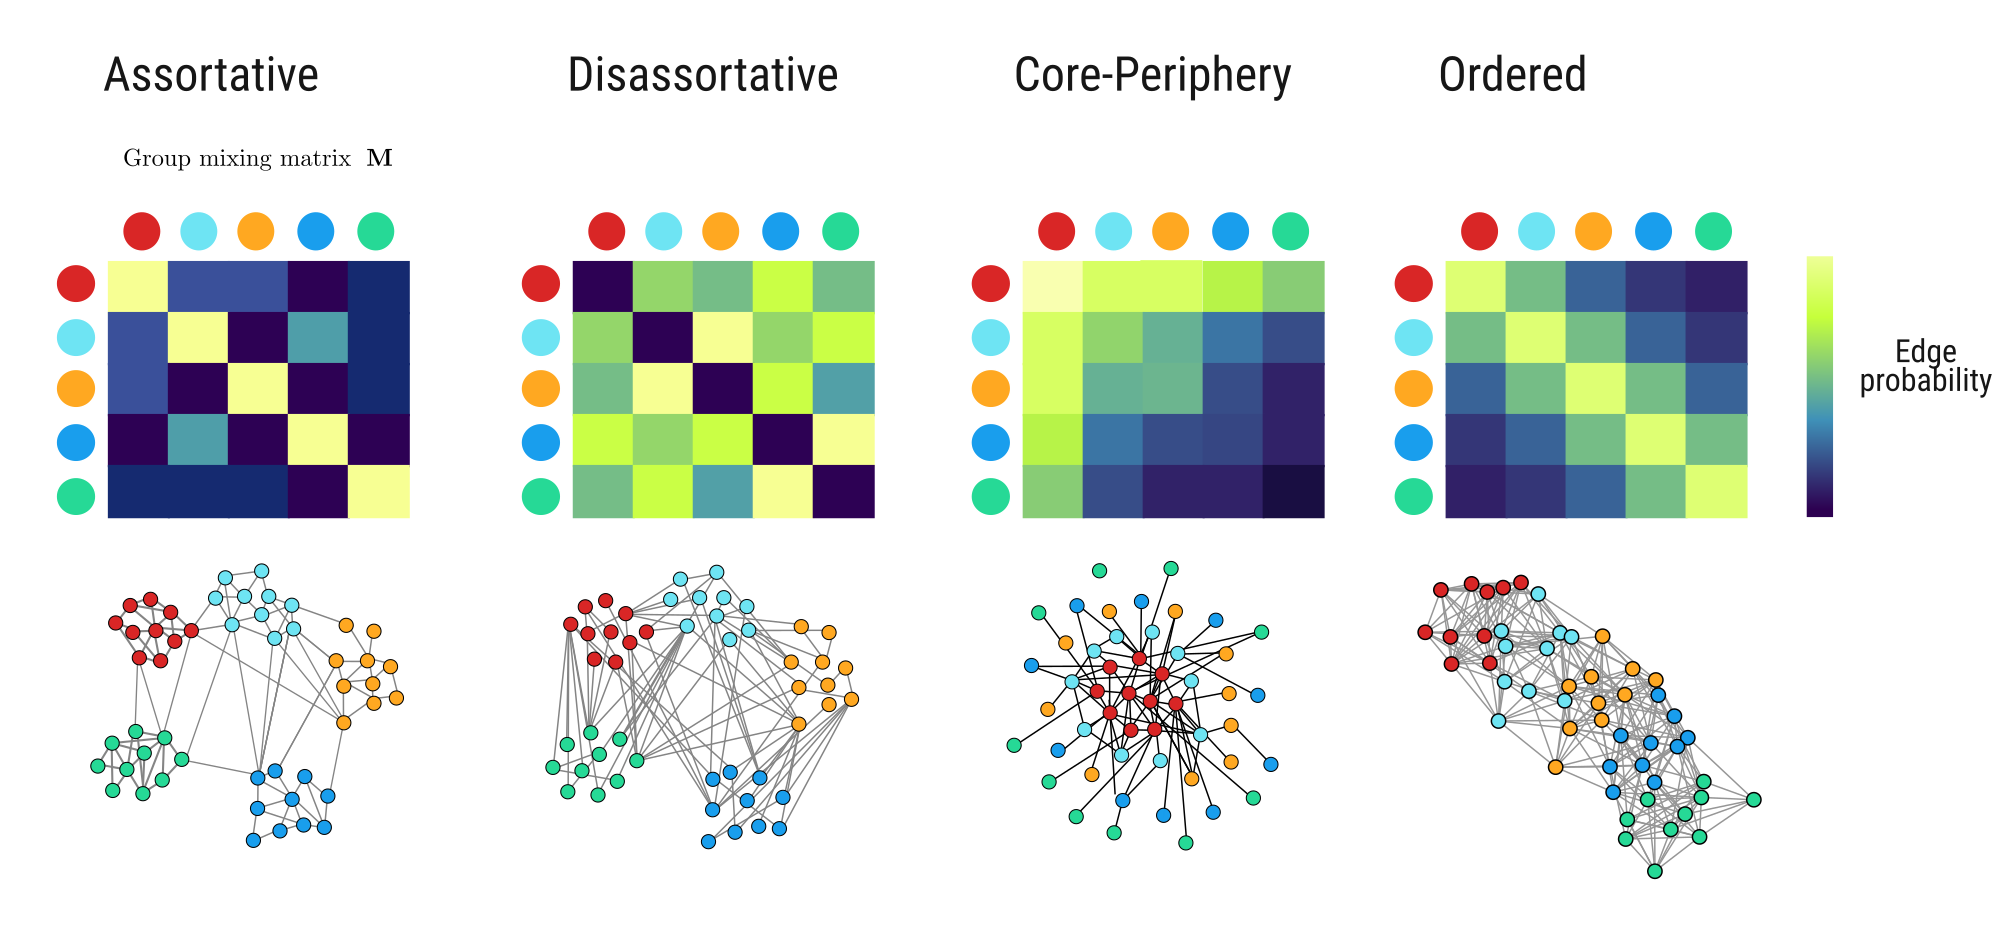
\includegraphics{./figures/blockmatrix.png}

}

\caption{Adapted from Clauset (2022). Shows how SBMs can account for
community structure beyond simple assortativity.}

\end{figure}

\hypertarget{how-do-we-infer-community-structure-from-stochastic-block-models}{%
\subsection{How do we infer community structure from stochastic block
models?}\label{how-do-we-infer-community-structure-from-stochastic-block-models}}

We can use Markov Chain Monte Carlo (MCMC) sampler to take an observed
matrix \(A\) and obtain an estimate of the posterior distribution of the
mixing matrix and group assignments,
\(P(\mathbf{M}, \vec{b} | \mathbf{A})\). To do this, we need to define
the likelihood of observing some network \(\mathbf{A}\) from a given
community partition \(\vec{b}\), and mixing matrix \(\mathbf{M}\). There
are differences in the best way to define both likelihood and priors
depending on underlying assumptions about network structure.

For unipartite networks, a common version is the Degree-Corrected SBM
(DC-SBM, Karrer \& Newman 2011), which explicitly accounts for the
degree distribution by including the empirical degree sequence in the
likelihood of observing each graph. Yen \& Larremore (2020) develops a
model specifically for bipartite networks, where the bipartite structure
is directly incorporated into the generative model, improving
performance for detecting communities in bipartite networks. Another
promising line of research is hierarchical/nested SBMs (NSBMs), first
proposed by Peixoto (2014). In NSBMs, each ``block''
\(\mathbf{M}_{b_i b_j}\) is \emph{itself} another SBM. This enables
multi-scale community detection that can circumvent the issue of
resolution limits from modularity maximization.

\hypertarget{conclusion}{%
\section{Conclusion}\label{conclusion}}

In summary, community detection is great, but modularity maximization is
useless. There are times when modularity, as a method of quantifying the
assortativity of edges in a graph given a set of group assignments
\(\vec{b}\), could correspond to an interesting ecological question.
However, using modularity \emph{as the criteria} to select the group
assignments is too unreliable to be the basis ecological conclusions. As
an alterative, we should use \emph{stochastic block models} to infer the
structure of modules within ecological networks.

\hypertarget{references}{%
\section*{References}\label{references}}
\addcontentsline{toc}{section}{References}

\hypertarget{refs}{}
\begin{CSLReferences}{1}{0}
\leavevmode\vadjust pre{\hypertarget{ref-Blondel2008FasUnf}{}}%
Blondel, V.D., Guillaume, J.-L., Lambiotte, R. \& Lefebvre, E. (2008).
\href{https://doi.org/10.1088/1742-5468/2008/10/P10008}{Fast unfolding
of communities in large networks}. \emph{Journal of Statistical
Mechanics: Theory and Experiment}, 2008, P10008.

\leavevmode\vadjust pre{\hypertarget{ref-Chung2002ConCom}{}}%
Chung, F. \& Lu, L. (2002).
\href{https://doi.org/10.1007/PL00012580}{Connected {Components} in
{Random Graphs} with {Given Expected Degree Sequences}}. \emph{Annals of
Combinatorics}, 6, 125--145.

\leavevmode\vadjust pre{\hypertarget{ref-Clauset2022LecNot}{}}%
Clauset, A. (2022). Lecture {Notes} -- {Network Analysis} and
{Modeling}.

\leavevmode\vadjust pre{\hypertarget{ref-Clauset2004FinCom}{}}%
Clauset, A., Newman, M.E.J. \& Moore, C. (2004).
\href{https://doi.org/10.1103/PhysRevE.70.066111}{Finding community
structure in very large networks}. \emph{Physical Review E}, 70, 066111.

\leavevmode\vadjust pre{\hypertarget{ref-Delmas2019AnaEco}{}}%
Delmas, E., Besson, M., Brice, M.-H., Burkle, L.A., Riva, G.V.D.,
Fortin, M.-J., \emph{et al.} (2019).
\href{https://doi.org/10.1111/brv.12433}{Analysing ecological networks
of species interactions}. \emph{Biological Reviews}, 94, 16--36.

\leavevmode\vadjust pre{\hypertarget{ref-Dormann2014MetDet}{}}%
Dormann, C.F. \& Strauss, R. (2014).
\href{https://doi.org/10.1111/2041-210X.12139}{A method for detecting
modules in quantitative bipartite networks}. \emph{Methods in Ecology
and Evolution}, 5, 90--98.

\leavevmode\vadjust pre{\hypertarget{ref-Fortunato2007ResLim}{}}%
Fortunato, S. \& Barthélemy, M. (2007).
\href{https://doi.org/10.1073/pnas.0605965104}{Resolution limit in
community detection}. \emph{Proceedings of the National Academy of
Sciences of the United States of America}, 104, 36--41.

\leavevmode\vadjust pre{\hypertarget{ref-Good2010PerMod}{}}%
Good, B.H., de Montjoye, Y.-A. \& Clauset, A. (2010).
\href{https://doi.org/10.1103/PhysRevE.81.046106}{The performance of
modularity maximization in practical contexts}. \emph{Physical Review
E}, 81, 046106.

\leavevmode\vadjust pre{\hypertarget{ref-Guimera2005FunCar}{}}%
Guimerà, R. \& Nunes Amaral, L.A. (2005).
\href{https://doi.org/10.1038/nature03288}{Functional cartography of
complex metabolic networks}. \emph{Nature}, 433, 895--900.

\leavevmode\vadjust pre{\hypertarget{ref-Hofman2008BayApp}{}}%
Hofman, J.M. \& Wiggins, C.H. (2008).
\href{https://doi.org/10.1103/PhysRevLett.100.258701}{Bayesian
{Approach} to {Network Modularity}}. \emph{Physical Review Letters},
100, 258701.

\leavevmode\vadjust pre{\hypertarget{ref-Holland1983StoBlo}{}}%
Holland, P.W., Laskey, K.B. \& Leinhardt, S. (1983).
\href{https://doi.org/10.1016/0378-8733(83)90021-7}{Stochastic
blockmodels: {First} steps}. \emph{Social Networks}, 5, 109--137.

\leavevmode\vadjust pre{\hypertarget{ref-Karrer2011StoBlo}{}}%
Karrer, B. \& Newman, M.E.J. (2011).
\href{https://doi.org/10.1103/PhysRevE.83.016107}{Stochastic blockmodels
and community structure in networks}. \emph{Physical Review E}, 83,
016107.

\leavevmode\vadjust pre{\hypertarget{ref-Lancichinetti2011LimMod}{}}%
Lancichinetti, A. \& Fortunato, S. (2011).
\href{https://doi.org/10.1103/PhysRevE.84.066122}{Limits of modularity
maximization in community detection}. \emph{Physical Review E}, 84,
066122.

\leavevmode\vadjust pre{\hypertarget{ref-Newman2004FinEva}{}}%
Newman, M.E.J. \& Girvan, M. (2004).
\href{https://doi.org/10.1103/PhysRevE.69.026113}{Finding and evaluating
community structure in networks}. \emph{Physical Review E}, 69, 026113.

\leavevmode\vadjust pre{\hypertarget{ref-Peixoto2014HieBlo}{}}%
Peixoto, T.P. (2014).
\href{https://doi.org/10.1103/PhysRevX.4.011047}{Hierarchical {Block
Structures} and {High-Resolution Model Selection} in {Large Networks}}.
\emph{Physical Review X}, 4, 011047.

\leavevmode\vadjust pre{\hypertarget{ref-Peixoto2021DesVs}{}}%
Peixoto, T.P. (2021).
\href{https://doi.org/10.1017/9781009118897}{Descriptive vs. Inferential
community detection in networks: Pitfalls, myths, and half-truths}.
\emph{arXiv.org}.

\leavevmode\vadjust pre{\hypertarget{ref-Yen2020ComDet}{}}%
Yen, T.-C. \& Larremore, D.B. (2020).
\href{https://doi.org/10.1103/PhysRevE.102.032309}{Community detection
in bipartite networks with stochastic block models}. \emph{Physical
Review E}, 102, 032309.

\end{CSLReferences}




\end{document}
